\refsubsection{Concepts}{subsec:concepts}
\todo{Graphs, eg. concept maps, co-occurrence graphs}
\todo{Classical text representations, eg.tfidf
Categories of algorithms, eg. algorithms on feature vectors, kernelized - algorithms}

\refsubsection{Definitions and Notations}{subsec:definitions_and_notations}
\todo{Lay groundwork for the later description of the problem}
\todo{Introductions to used classifiers, concepts}
\todo{Concretize the problem and its notation}
\todo{Comparison of the used data sources}

\subsubsection{Classification Task}
\todo{Supervised}

\subsubsection{Graphs}
A graph is a triple $G = (V, E, L)$, where $V$ is the set of vertices, $E \subset V \times V$ are the edges and $L: V \to X$ is a labeling function which assign a labels from some space $X$ to a given node.

A graph is called undirected when $\forall (v_1, v_2) \in E: (v_2, v_1) \in E$, otherwise it is called directed.

The neighbours $n(v)$ of a node $v$ are defined as $n(v) = \{v' | (v, v') \in E \}$.


\todo{Degree, centrality, random-walk, ...}
%The in-degree $degree_{in}$ of a vertex $v \in V$ is $degree_{in}(v) = |\{v | (v_1, v_2) \in E \land v_2 = v\}|$.
%The out-degree $degree_{out}$ is analogously defined as $degree_{out}(v) = |\{v | (v_1, v_2) \in E \land v_1 = v\}|$.
%The degree of a vertex $v$ is $degree(v) = degree_{in}(v) + degree_{out}(v)$ for directed graphs, and $degree(v) = degree_{in}$ for undirected graphs.

A walk on a graph is a (finite) sequence of edges, $w = (e_1, \cdots, e_n)$ with the constraint that $\forall e_i = (v_1, v_2) \in w: \exists v_3: e_{i + 1} = (v_2, v_3)$.
The set of all possible walks is denoted $W$.

A path is a walk with the constraint that every node is visited at most once.
The set of all possible paths is denoted $P$.

The distance $d(v_1, v_2)$ between two vertices is defined as the length of the shortest path between them.

A connected component $c$ of a graph is a set of vertices with the constraint $\forall v, v' \in c: \exists p \in P: v \in p \land v' \in p$, ie. a path between the two vertices exists.



\paragraph{Concept Map}
A concept map is a (directed) graph where the nodes are concepts.
Concepts are tokens in a text.
Concepts consist of one or more words.
A directed edge between two concepts show that these concepts are related to each other. The edges can have labels, too.
For an example of a concept map, see Figure \ref{fig:concept_map}.

\begin{figure}[h]
\centering
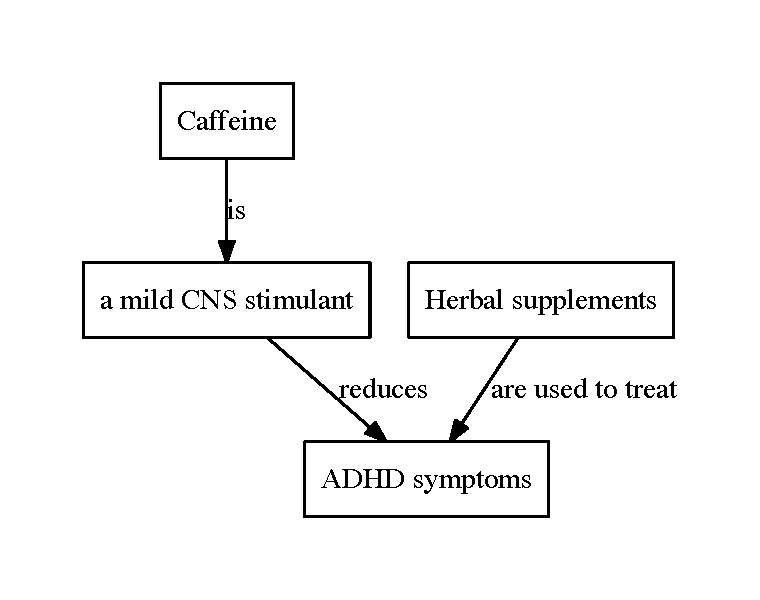
\includegraphics[width=0.5\linewidth]{assets/figures/concept_map.pdf}
\caption{Example of a concept map. The nodes are the concepts. The directed edges connect the concepts to each other and have labels. In this example of a concept map, one could recover sentences from this graph, for example ``Caffeine \textit{is} a mild CNS stimulant". Taken and adapted from: \cite{Falke2017}}
\label{fig:concept_map}
\end{figure}

Concept maps are useful for visualizing concepts and their relation to each other.
Concept maps can thus be used to quickly explore a given topic and immediately see connections between concepts.
Through the degree of a concept, one can also infer the relative importance of that concept in the underlying text.

By combining different texts of the same topic, one can also create a concept map for that topic - the concepts are not confined to a single text in this case.
The visualization with concept maps of one or more individual texts therefor enables the non-linear exploration of multiple texts of a topic.

Because the concepts in a concept map often contain only a small subset of the text, concept maps also summarize the underlying text.
Only relevant concepts and their relation to each other are captured, making concept maps interesting for (multi-document) text summarization, too.

In Chapter \ref{sec:implementation} we introduce the concept map extraction implementation we used and further explain the steps in creating the concept maps.

\todo{"Capture important concepts and the structure of texts (spanning over whole text)"}
\todo{Advantages}
\todo{Text summarization}

\paragraph{Co-Occurrence Graph}
A co-occurrence graph, or graph-of-words, is generated from a text by creating a (undirected) graph with the words of the text as nodes.
There is an edge between two nodes if their labels co-occur in the text.
Two words co-occur when the distance between the words in the text is below a given threshold, the window size.

In Figure \ref{fig:cooccurrence_graphs} are examples of co-occurrence graphs for the sentence: .

\begin{figure}[ht]%
    \centering
    \subfloat[Window size: 1]{{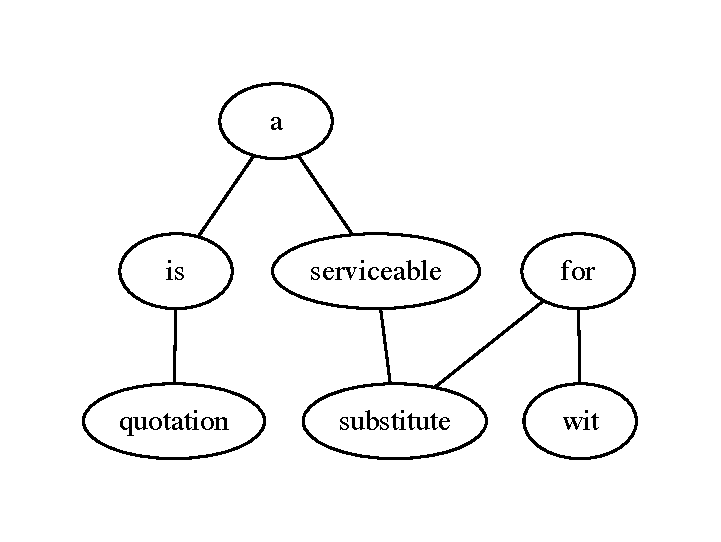
\includegraphics[width=0.3\textwidth]{assets/figures/cooccurrence_graph_1.pdf} }}%
    \subfloat[Window size: 2]{{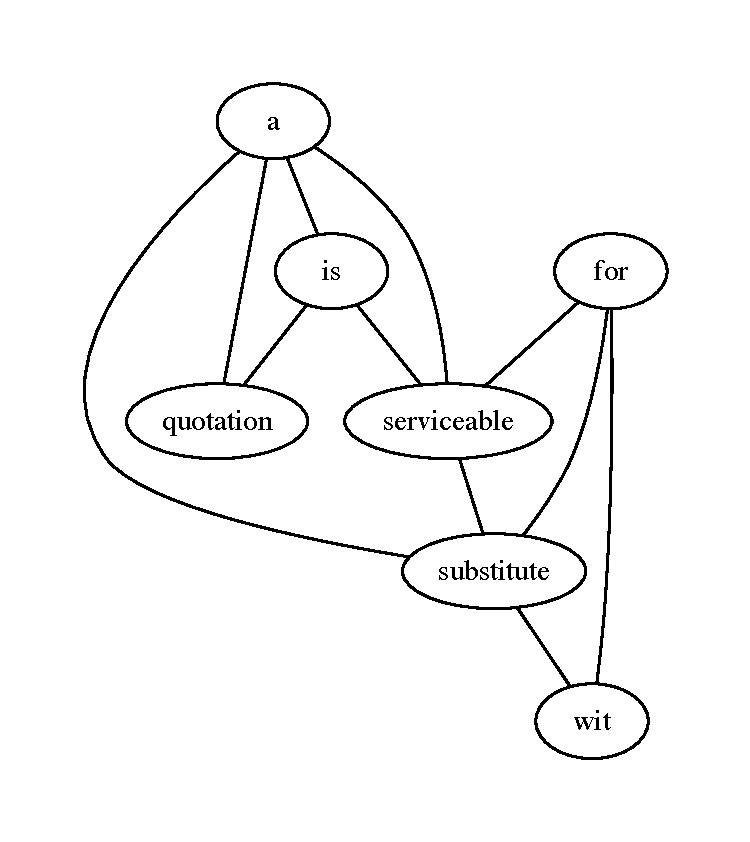
\includegraphics[width=0.3\textwidth]{assets/figures/cooccurrence_graph_2.pdf} }}%
    \subfloat[Window size: 3]{{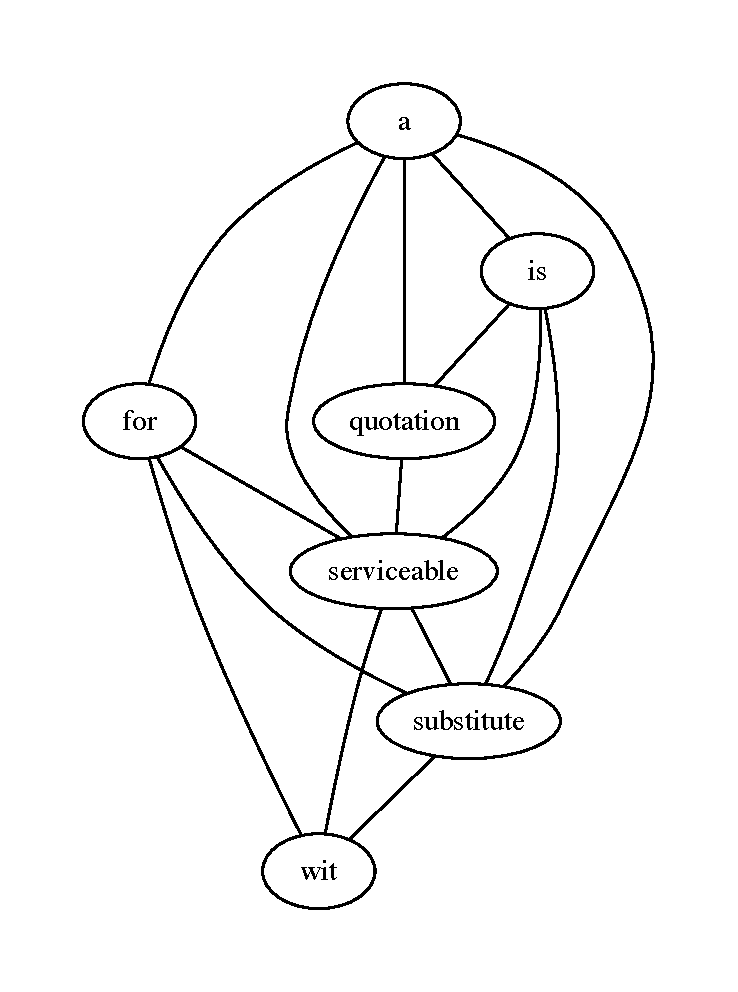
\includegraphics[width=0.3\textwidth]{assets/figures/cooccurrence_graph_3.pdf} }}%
    \caption{Example for co-occurrence graphs. Generated from the sentence: ``Quotation is a serviceable substitute for wit". Different window sizes.}%
    \label{fig:cooccurrence_graphs}%
\end{figure}

Co-occurrence graphs not only contain the words of the underlying text but also their co-occurrence.
For a window size of $w$, they capture n-grams of size $n \leq w$.

\subsubsection{Graph kernel}
In most cases, texts and graphs are of non-fixed size. 
However, most classification algorithms require fixed size vectors to operate on.
In graph classification, the number of the nodes and edges per graph is also not fixed.
Nevertheless, there are several approaches to overcome this problem and enable graph classification.
One of these approaches are so-called graph kernels.

A graph kernel is a function $k$ which returns a measure of similarity between two graphs:
\begin{equation*}
k: G \times G \rightarrow \mathbb{Q}
\end{equation*}

The graph kernel function has to be:
\begin{itemize}
    \item{\textit{symmetric}: $k(G_1, G_2) = k(G_2, G_1)$}
    \item{\textit{non-negative definite}: \dots}
\end{itemize}

Graph kernels can be used in kernel methods for classification and other tasks.
Prominent examples of kernel methods are the SVM, kernelized PCA and Gaussian Processes.

For a subset of graph kernels, one can also create explicit feature vectors for the graphs. In this case, the kernel can be written as an inner product on two fixed-size vectors:
\begin{equation*}
    k(G_1, G_2) = \langle \phi(G_1), \phi(G_2) \rangle
\end{equation*}
Here, $\phi(G)$ returns a fixed-size vector representation of graph $G$.
This $\phi(G)$ can be used in all vector-based classification algorithms, not only kernel methods.

\paragraph{Example}
As an example we will investigate a simple graph kernel which actually discards all structural information about the graph. This graph kernel only operates on the labels of the nodes:
\begin{equation*}
k_{common\_label}(G_1, G_2) = | l(G_1) \cap l(G_2) |
\end{equation*}
where $l(G)$ returns the set of labels for graph $G$.
Therefor, this graph kernel counts the number of common labels of the two graphs. Two graphs are similar if they have the same node labels.
An extension to this graph kernel is using the Jaccard coefficient instead of just counting the common node labels:
\begin{equation*}
k_{common\_label\_jaccard}(G_1, G_2) = \frac{| l(G_1) \cap l(G_2) |}{| l(G_1) \cup l(G_2) |}
\end{equation*}
This extension normalizes the function and confines the codomain of $k$ to $[0, 1]$.

Another example for a graph kernel which only operates on the structure of the graph is the following:
\begin{equation*}
k_{simple\_structure}(G_1, G_2) = 
\end{equation*}
%where $c(G)$ returns the number of connected components of $G$, and $d(G)$ returns the average degree

Several graph kernels have been proposed in the literature.
Categories of graph kernels include graph kernels based on shortest-paths, random-walks, 
Graph kernels can be categorized coarsely into graph kernels based on shortest-paths, random-walks and subtree patterns.

\todo{Categories of graph kernels, eg. random-walk-based, subtree-based}
\todo{Graph kernels can be combined!}
\todo{Simple graph kernel, eg. simple-label-matching or jaccard}
\todo{Examples of graph kernels}
\todo{Mention similarity of graph kernel task to graph isomorphism test}
\todo{Explain when $\phi$ can be constructed (Mercer's theorem: an implicitly defined function $\varphi$  exists whenever the space $\mathcal{X}$ can be equipped with a suitable measure ensuring the function $k$ satisfies Mercer's condition.)}

\paragraph{Gram matrix}
A gram or kernel matrix for a given kernel is a matrix $A$ where the entries are the pairwise similarities of graphs:
\begin{equation*}
    A_{i,j} = k(G_i, G_j)
\end{equation*}
The gram matrix is symmetric by definition since the underlying kernel is also symmetric, so $A_{i,j} = A_{j, i}$.

\subsubsection{Kernel Methods and Kernel trick}



\refsubsection{Related Work}{subsec:related_work}
\todo{How did the field evolve?}
\todo{Hint related tasks}
\todo{What is the most related work, how do they differ from our approach
Relate the other work to the new approach and work out their differences/results}
\todo{Other approaches to graph classification}
\todo{Mention other graphs}

\paragraph{``Shortest-Path Graph Kernels for Document Similarity" \cite{Nikolentzos2017a}}
The most similar and recent approach to our approach that we found was \cite{Nikolentzos2017a}. In this paper, the authors first create co-occurrence graphs out of the text, then run their own graph kernel on top of them. They create a gram matrix and use a SVM to classify the graphs. Their graph kernel consists of three parts:
\begin{enumerate}
\item{Simple label matching: the number of matching node labels are compared between the two graphs}
\item{Shortest path: generate a shortest-path graph}
\end{enumerate}

\paragraph{``Text Categorization as a Graph Classification Problem" \cite{Rousseau2015a}}
Co-occurrence graphs out of text corpus

``Subgraphs as features": extraction of k-core (or main-core), then most-frequent subgraph mining

Datasets: r8 (subset), webkb (subset), ling-spam, amazon

First real evaluation of graph-based classification with a high number of graphs/unique nodes/... - promising results

Only using the most-important subgraph of a graph (main core) does not greatly damage prediction accuracy, but substantially reduces compute time

\paragraph{``Concept Graph Preserving Semantic Relationship for Biomedical Text Categorization" \cite{Gulrandhe2015}}
